\chapter{Increasing Your Value}

This chapter follows a Jim Rohn lecture preserved in a curated playlist rather than in a formal institutional course. We keep close to the spoken order because the lecture is built as a deliberate chain: first a law of self-change, then a way to measure it, then a correction about value and time, then a ladder model of income, and only after that the autobiographical proof and the closing rule about working on oneself. Curation credit for the playlist belongs to LazyingArt LLC.

\section{Opening Formula and the Adventure of Personal Development}

The lecture opens with a sentence that sounds motivational until we notice that it governs everything that follows:

\begin{equation}
\text{Everything changes for you} \Longleftarrow \text{You change}.
\end{equation}

Rohn immediately explains the direction of the implication. We do not first change what is outside. We change what is inside. That is why the next step tightens the same claim into a more operational form:

\begin{equation}
\text{Have More} \Longleftarrow \text{Become More}.
\end{equation}

This is the lecture's master variable. Wages, promotions, opportunities, and even the style of one's future will later be treated as consequences of this first relation. That is why the lecture begins with the paired admonitions: do not wish it were easier; wish you were better. Do not wish for fewer problems; wish for more skills. The speaker is relocating causality from environment to person.

He then gives the theme its explicit name: personal development. What matters here is that he does not present it as an abstract chapter heading. He presents it as an ``extraordinary adventure'' that began for him at age twenty-five and has not ended. He wants his craft to get better, his business operations to get better, the things he does to get better. Once he picked up what he calls the simple formula, he says, it became easy to see where the problem was if one would go to work on it.

That transition matters. The lecture has not yet become economic. It has only established the law to which the later economics will answer.

\section{Why Start with Money? Counting as a Diagnostic}

Only after the opening law is in place does Rohn ask how we might explain personal development concretely. His answer is pragmatic: start with money. Not because money is the only value, and not because economics is the whole of life, but because money is countable.

\begin{equation}
\text{Money}=\text{a first countable diagnostic, not the whole of value}.
\end{equation}

The lecture slows down here for a reason. It wants to justify its method before it begins using it. Some things are hard to measure. Money is not. Somebody asks, ``How are you doing?'' and the speaker's almost comic answer is, ``Let's count.'' The point is not reductionism. The point is that if we want to detect lack of discipline, judgment, or development, then a countable variable is a sensible place to begin.

This is one of the lecture's quieter pivots. We move from the broad law of self-change to a narrow test case where consequences show up numerically. Only then does Rohn narrow into the chapter's real mathematical hinge.

\section{Value, Time, and the Marketplace}

The key economic sentence is introduced with pedagogical force: we get paid for bringing value to the marketplace. Rohn then adds a second gloss that hardens the first. Marketplace, he says, is also called reality.

\begin{equation}
\text{Marketplace}=\text{Reality}.
\end{equation}

\begin{figure}[h]
\centering

\includegraphics[width=.78\linewidth]{lecture_17_figure_02.png}
\caption{Flipchart contrasting value and time. The board words are only partly legible, but \emph{Value}, \emph{time}, and a likely gloss toward \emph{reality} are visible.}
\end{figure}

The flipchart is useful here because it preserves the board layout of the distinction even when the handwriting is not fully recoverable. The large word is \emph{Value}; the smaller note is \emph{time}; the lower parenthetical note appears to point toward \emph{reality}. We should not over-transcribe what is blurry, but we do have enough to place a clean reconstruction nearby.

\subsection{Question \& Answer}

\paragraph{Question.} Do we get paid for time or for value?

\paragraph{Answer.} We get paid for value. Time is required to bring value to the marketplace, but time itself is not what is being bought.

The lecture's correction may therefore be written as

\begin{align}
\text{Pay} &\neq \text{Time alone},\\
\text{Pay} &\propto \text{Value brought to the marketplace}.
\end{align}

The spoken sequence is important and should remain visible in the notes. First, Rohn grants that it takes time to bring value to the marketplace. Then he blocks the common misunderstanding that one is literally ``making so much an hour.'' ``Not true,'' he says twice, and the repetition carries the structure. If the hour itself were the thing being bought, then one could stay home and have the money sent over. The hour is only the medium. Value is the content.

That is why the lecture compresses the relation one step further into a sentence that sounds almost like a theorem:

\begin{equation}
\text{You get paid for the value you put in the time}.
\end{equation}

A narrow reconstruction of the board logic is therefore useful:

\begin{figure}[h]
\centering
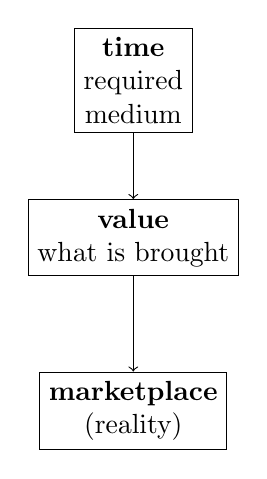
\begin{tikzpicture}
\node[draw, align=center] (t) at (0,2.9) {\textbf{time}\\required\\medium};
\node[draw, align=center] (v) at (0,0.9) {\textbf{value}\\what is brought};
\node[draw, align=center] (m) at (0,-1.3) {\textbf{marketplace}\\(reality)};
\draw[->] (t) -- (v);
\draw[->] (v) -- (m);
\end{tikzpicture}
\caption{Transcript-derived reconstruction of the lecture's value-time-marketplace relation.}
\end{figure}

Now the lecture is ready to ask its first explicit quantitative question.

\section{Multiplying Value in the Same Time}

Once value has replaced time as the active variable, the lecture immediately tests the consequence. If we are paid for value, and if time is held fixed, can we become twice as valuable and make twice as much money in the same time? Can we become three times as valuable and make three times as much money in the same time?

\subsection{Question \& Answer}

\paragraph{Question.} Is it possible to make more money in the same time?

\paragraph{Answer.} Yes. If we raise the value brought to the marketplace while holding time fixed, then pay can rise with it.

Rohn's answer is emphatic: ``Of course. Of course.'' We can preserve the operational content with a minimal piece of notation. Let \(T\) denote time, \(V\) value, and \(P\) pay. This is not meant as a full economic theory. It is a clean way to expose the lecture's spine. Holding \(T\) fixed, we write

\begin{align}
P &= kV,\\
V_2 = 2V_1 \quad &\Longrightarrow \quad P_2 = 2P_1,\\
V_3 = 3V_1 \quad &\Longrightarrow \quad P_3 = 3P_1.
\end{align}

The point is not the constant \(k\). The point is that once the lecture has corrected the variable, the rest follows by direct implication. More money in the same time does not require more clock. It requires more value. That is why the section closes on the lecture's own summary:

\begin{equation}
\text{Earn more money in the same time} \Longleftarrow \text{Become more valuable}.
\end{equation}

The narrative rhythm is important here. The puzzle is asked only after the value-time distinction is established, and the answer matters because it becomes the rule governing everything after it.

\section{The Ladder, Marketplace Reality, and the Question of More Money}

The lecture now changes register. We move from a cleaned relation to a public picture. America, Rohn says, is a ladder to climb. It is not a bed. The metaphor matters because it converts a question about wages into a question about motion.

\begin{equation}
\text{America is a ladder to climb}.
\end{equation}

\begin{figure}[h]
\centering

\includegraphics[width=.62\linewidth]{lecture_17_figure_03.png}
\caption{Flipchart wage example near \(\$4\) an hour. The writing is fragmentary, but the visible numeric mark supports the starting-rung discussion.}
\end{figure}

The board fragment does not preserve a visible ladder, so we should not claim one. What it does preserve is the numeric starting-point example around \(\$4\) an hour. The transcript makes the context secure enough for a cautious reconstruction:

\begin{equation}
\text{Start at } \$4/\text{hour}.
\end{equation}

Rohn uses this to answer the political complaint that the starting place ``should be five.'' His answer is not really about legislation. It is about the geometry of the metaphor. A ladder is for climbing. If one intends to remain forever on the bottom rung, then perhaps five matters enormously. But if one intends to climb, then the central question is different.

\begin{equation}
\$4 \to \$5 \to \cdots
\end{equation}

\begin{figure}[h]
\centering
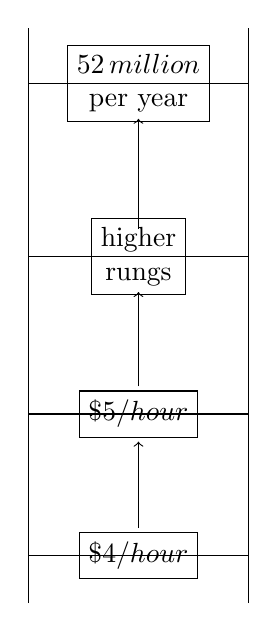
\begin{tikzpicture}
\node[draw, align=center] (r1) at (0,0.0) {\(\$4/\text{hour}\)};
\node[draw, align=center] (r2) at (0,1.8) {\(\$5/\text{hour}\)};
\node[draw, align=center] (r3) at (0,3.8) {higher\\rungs};
\node[draw, align=center] (r4) at (0,6.0) {\(52\,\text{million}\)\\per year};
\draw (-1.4,-0.6) -- (-1.4,6.7);
\draw ( 1.4,-0.6) -- ( 1.4,6.7);
\draw (-1.4,0.0) -- (1.4,0.0);
\draw (-1.4,1.8) -- (1.4,1.8);
\draw (-1.4,3.8) -- (1.4,3.8);
\draw (-1.4,6.0) -- (1.4,6.0);
\draw[->] (0,0.35) -- (0,1.45);
\draw[->] (0,2.15) -- (0,3.35);
\draw[->] (0,4.15) -- (0,5.55);
\end{tikzpicture}
\caption{Transcript-derived ladder reconstruction. The screenshot preserves the starting-rung example; the ladder itself is reconstructed from the spoken lecture.}
\end{figure}

The lecture then widens its scale. The more valuable we become, the higher we move up the ladder. That is why the example jumps from \(\$4\) an hour to top executive compensation and then to the sharper question of why anyone would be paid \(\$400\) an hour. The answer is always the same: because the person has become that valuable to the marketplace.

\subsection{Question \& Answer}

\paragraph{Question.} How do we get more money?

\paragraph{Answer.} Not by treating the ladder as a bed, and not by demanding a richer bottom rung while remaining the same. We get more money by becoming more valuable and climbing.

This is where the lecture makes one of its hardest distinctions. A person may be valuable as a brother, as a member of the community, as a member of the church, in the sight of God, and to the human family, and still not be very valuable to the marketplace. The point is not that human value and economic value are the same. It is that they are not the same, and that wages answer to the narrower one.

That is why the lecture can record the pair of implications

\begin{align}
\text{Low marketplace value} &\Longrightarrow \text{Low marketplace pay},\\
\text{High marketplace value} &\Longrightarrow \text{High marketplace pay}.
\end{align}

And that is why it rejects false strategies in such compressed form:

\begin{align}
\text{Demand} &\not\Longrightarrow \text{Riches},\\
\text{Waiting for a raise} &< \text{Climbing by added value}.
\end{align}

At this point the lecture has completed its economic argument. Everything that remains is proof and return.

\section{The Phone Call Worth Millions and Shoaff's Secret}

The next move is autobiographical, but it is not a digression. Rohn tells the story of a phone call from a company ready to expand internationally, a call that would add millions to his fortune. At first the fact that they called him appears surprising. Then comes the second thought: of course they called him. Who else would they call if he could get the job done?

The anecdote is the lecture's narrative verification of the earlier equations:

\begin{equation}
\text{Telephone call worth millions} \Longleftarrow \text{I had become valuable}.
\end{equation}

The biographical contrast is essential and should remain strong. Farm boy from Idaho. Raised in obscurity. One year of college. Creditors calling at age twenty-five. Pennies in pocket. Nothing in the bank. Promises behind. How can such a person later receive a call worth millions? The lecture insists on the answer twice: he changed.

That story folds directly into Shoaff's secret. Learn to work harder on your life, and in particular harder on yourself, than you do on your job. In this form the lecture reaches its most concise pair of rules:

\begin{align}
\text{Work hard on your job} &\Longrightarrow \text{Make a living},\\
\text{Work hard on yourself} &\Longrightarrow \text{Make a fortune}.
\end{align}

But even here the lecture does not let ``fortune'' remain merely monetary. The closing movement widens again to philosophy, attitude, personality, language, communication, and ability. Economics was the first measuring stick, not the final horizon. That is why the closing recurrence of the central rule should remain two-layered:

\begin{equation}
\text{Make yourself more valuable to the marketplace} \Longrightarrow \text{Change in income},
\end{equation}

and beyond that, more broadly,

\begin{equation}
\text{Work on the inside} \Longrightarrow \text{The outside becomes easier to change}.
\end{equation}

Rohn closes by making the implication practical: promotions, money, economics, future---these stop looking like separate problems once we are working on the right variable.

\section{Summary}

The lecture begins with a law of self-change, narrows into a countable test case, and then builds an economic chain from that law. We first replace time by value as the decisive marketplace variable. We then ask what happens if value rises while time is held fixed. From there we move into the ladder image, where the point is not merely to negotiate the bottom rung but to climb. Then the lecture separates marketplace value from other forms of value, rejects demand and passive waiting as false strategies, and verifies the whole structure through the phone call worth millions.

What makes the lecture coherent is that it never abandons its opening axiom. The economic sequence is not a detour away from personal development. It is the first sharp illustration of it. The chapter should therefore end exactly where the lecture wants us to end:

\begin{equation}
\text{Everything changes for you} \Longleftarrow \text{You change}.
\end{equation}